\documentclass[a4paper,12pt]{article}

\usepackage[margin=2.5cm]{geometry}
\usepackage[T1]{fontenc}
\usepackage[utf8]{inputenc}
\usepackage[danish]{babel}
\usepackage{listings}
\usepackage{graphicx}
\graphicspath{{figures/}}
\setlength{\parindent}{0cm}
\setlength{\parskip}{1em}

\title{Programmering og Problemløsning\\Datalogisk Institut,
  Københavns Universitet\\Uge(r)seddel 1 - gruppeopgave}
\author{Jon Sporring}
\date{5.\ september - 14.\ september}

\begin{document}
\maketitle

Velkommen til kurset ``Programmering og Problemløsning''.

Dette er den første af i alt~12 \emph{uge(r)sedler}. Uge(r)sedlerne indeholder information om opgaver samt diverse praktisk information og perspektivering af ugens/ugernes pensum. Vi har 16 undervisningsuger, og de fleste sedler vil gælde 1 uge, men som denne vil nogle strække sig over flere uger.

Denne ugeseddel gælder for perioden 5/9 til 14/9. Pensum angives under "`Forelæsnings- og læseplan"' på Absalon og materialet finder i under Absalonpunktet "`Noter, links, software m.m."'.  I denne periode skal I arbejde i grupper. Formålet er at:
\begin{itemize}
\item stifte bekendtskab med imperativ programmering gennem Scratch
\item lave et spil
\item stifte bekendtskab med kommandoterminalen og filstrukturer
\item stifte bekendtskab med en teksteditor
\item skrive en rapport i LaTeX og lave den første Absalon aflevering
\end{itemize}

Denne uges opgaver er specificeret nedenfor. Husk at processen og resultatet skal dokumenteres til sidst, så det er en god ide at tage udførlige noter undervejs. Opgaven lyder:
\begin{description}
\item[1.0] Start Scratch, og lav et lille program, som flytter katten (eller en anden sprite) rundt på skærmen vha.\ glide-blokken og gentagelse.
\item[1.1] Hvad kan I lave med 10 blokke?\\
  I Figur~\ref{fig:blokke} ser I 10 Scratch blokke.
  \begin{figure}
    \centering
    
\includegraphics[height=0.04\paperheight]{glide.png}
    
\includegraphics[height=0.04\paperheight]{go.png}
    
\includegraphics[height=0.04\paperheight]{hide.png}
    
\includegraphics[height=0.04\paperheight]{playSound.png}
    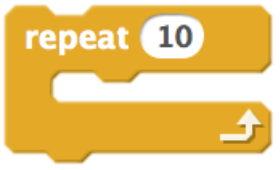
\includegraphics[height=0.08\paperheight]{repeat.png}
    
\includegraphics[height=0.045\paperheight]{say.png}
    
\includegraphics[height=0.04\paperheight]{setSize.png}
    
\includegraphics[height=0.04\paperheight]{show.png}
    
\includegraphics[height=0.04\paperheight]{wait.png}
    
\includegraphics[height=0.055\paperheight]{when.png}
    \caption{10 Scratch-blokke}
    \label{fig:blokke}
  \end{figure}
  Jeres opgave er at lave et sjovt program, kun ved brug af disse blokke. Hver blok må bruges 0, 1 eller flere gange. Prøv at sammensætte programmet ved at tegne blokkene på papir, og skriv ned, hvad I tror programmet vil gøre. Sæt jer dernæst til computeren, og indtast jeres program. Beskriv, i hvor høj grad programmet gør, som I forventede. Vend dernæst tilbage til designfasen og forbedre evt.\ programmet. Til slut uploades programmet til gruppens rum i Scratch.
\item[1.2] Design et spil\\
  I skal designe og implementere et spil efter eget valg. Spillet skal indeholde 2-5 sprites, vare ca.\ 1 minut at spille og må benytte alle tilgængelige blokke i Scratch. Det må gerne minde om et spil I kender, og det er ikke vigtigt at det er et grafisk eller lydmæssigt prangende spil. Start med at tale om hvad I kunne tænke jer, spillet skal omhandle. Skitser på papir, hvordan game-playet, skal forløbe. Skitser derefter på papir hvordan det kunne implementeres i Scratch. Indtast programmet på computeren og afprøv, om spillet gør, som I forventer. Vend tilbage til designfasen og forbedre evt. spillet.
\end{description}
Programmerne udviklet i Opgave 1.1 og 1.2 skal afleveres ved at dele i klassens rum i Scratch, og processen og et passende antal skærm-dumps dokumenteres ved at skrive en rapport i LaTeX. Både LaTeX koden og den oversatte pdf fil afleveres i Absalon.

Til øvelserne forventer vi at I arbejder efter følgende skema:
\begin{description}
\item[Mandag 5/9:] Opgave 1.0 og 1.1
\item[Tirsdag 6/9:] Opgave 1.1, hvis I ikke blev færdige, og start på Opgave 1.2
\item[Fredag 9/9]  Opgave 1.2
\item[Mandag 12/9] Opgave 1.2
\item[Tirsdag 13/9] Rapportskrivning i LaTeX.
\end{description}

\flushright God fornøjelse.
\end{document}

%%% Local Variables:
%%% mode: latex
%%% TeX-master: t
%%% End:
